%\begin{figure*}[t]
%\centering
%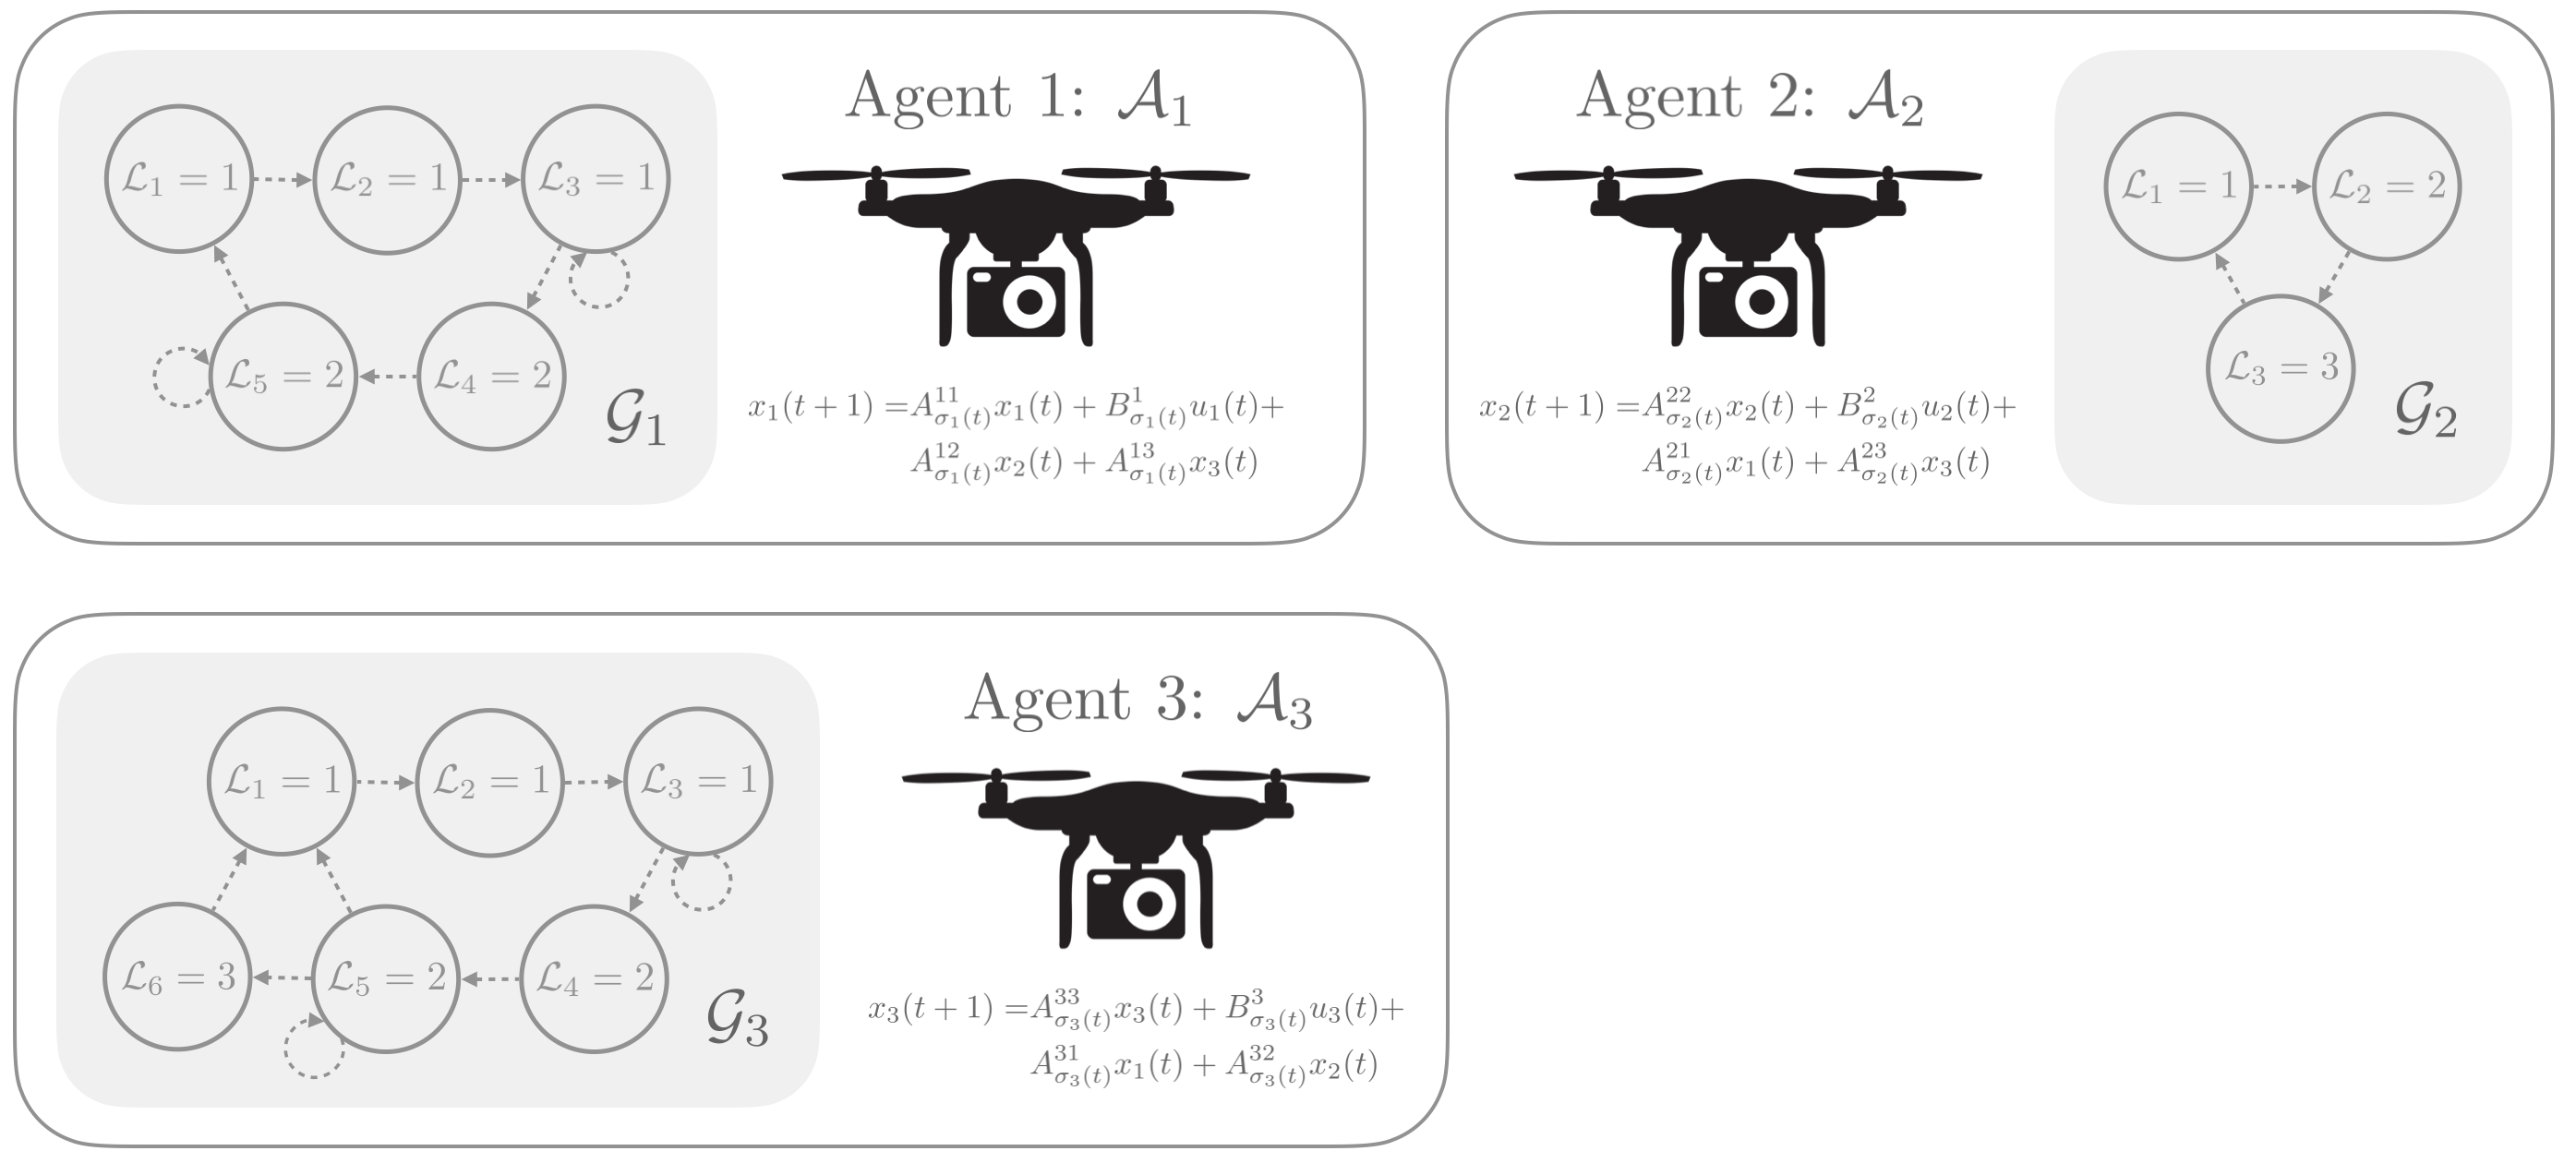
\includegraphics[width=\textwidth]{./figures/sample_system}
%\end{figure*}

\section{System Description}
In the previous sections, the systems have only contained a single switching signal. In general, however, systems may contain many switching signals. Consider a collection of $\numagents\in\int\rgeq{1}$ external switching signals each respecting their own directed graph, $\ssl[\agentidx](t)\in\Sigma(\graph^\agentidx)\ \agentidx\in\idxset{\numagents}$. Further, consider a system with all these signals and dynamics taking the form
\begin{align}
A(t)&=\begin{bmatrix}
A^{11}_{\ssl[1](t)}&A^{12}_{\ssl[1](t)}&\cdots&A^{1\numagents}_{\ssl[1](t)},\\
A^{21}_{\ssl[2](t)}&A^{22}_{\ssl[2](t)}&\cdots&A^{2\numagents}_{\ssl[2](t)},\\
\vdots&\vdots & \ddots & \vdots\\
A^{\numagents 1}_{\ssl[\numagents](t)} & A^{\numagents 2}_{\ssl[\numagents](t)} &\cdots & A^{\numagents \numagents}_{\ssl[\numagents](t)} 
\end{bmatrix},\\
B(t)&=\begin{bmatrix}
B^{1}_{\ssl[1](t)}&0&\cdots&0,\\
0&B^{2}_{\ssl[2](t)}&\cdots&0,\\
\vdots&\vdots & \ddots & \vdots\\
0 & 0 &\cdots & B^{\numagents}_{\ssl[\numagents](t)} 
\end{bmatrix},\\
\xcon(t)&=\xcon[\ssl[1](t)]^1\times\cdots\times\xcon[\ssl[\numagents](t)]^\numagents,\\
\ucon(t)&=\ucon[\ssl[1](t)]^1\times\cdots\times\ucon[\ssl[\numagents](t)]^\numagents.
\end{align}
This structure is motivated by distributed systems with coupling in the system's states. Note how each block-row is governed by a single switching signal. This makes intuitive sense because local switching signals are more likely to effect how neighboring states impact the local agent rather then how local states will effect neighboring agents.

The objective of this work is to design a safe-set collection for systems with the above structure. A naive solution would simply be to define a new switching signal with states corresponding to all the realizable permutations of the independent signals. While this would work in theory, it creates an exponential growth in the cardinality of the safe-set collection. A second challenge arrizes when the probable size of the state space is considered. Having even just three block-rows of three dimensions each leads to a six dimension system and will tax the naive implementation. These concerns will be addressed by splitting the system into block-rows and looking for safe-set collections, $\mathcal{S}^{\agentidx}=\{\mathcal{S}^\agentidx_n\}_{n\in\gnumnodes[\agentidx]}$, for each separately. Once found, the collections can be merged into a large collection with all possible switching signal states represented.

\subsection{Block-row Dynamics}
Looking only at the block row indexed by $\agentidx$, the dynamics can be rewritten as 
\begin{align}\label{eq:block-row-dyn}
x_\agentidx(t+1)&=A^{\agentidx\agentidx}_{\ssl[\agentidx](t)}x_\agentidx(t)+B^\agentidx_{\ssl[\agentidx](t)}u_\agentidx(t)\nonumber\\&\quad+\sum_{\tilde\agentidx\in\idxset{\numagents}\setminus \agentidx}A^{\agentidx\tilde\agentidx}_{\ssl[\agentidx](t)}x_{\tilde\agentidx}(t)\\
=A^{\agentidx}_{\ssl[\agentidx](t)}&x_\agentidx(t)+B^\agentidx_{\ssl[\agentidx](t)}u_\agentidx(t)+E_{\ssl[\agentidx](t)}^\agentidx w(t),
\end{align}
with $w(t)\in\wcon[\ssl[\agentidx](t)]^\agentidx$. The existence of $\wcon[\ssl[\agentidx](t)]^\agentidx$ can be inferred from the fact that the full system is constrained. These dynamics and constraints are collected into the following tuple defining agent $\agentidx$,
$$\agent{\agentidx}\triangleq\{\{A^{\agentidx}_{\modeidx},B^\agentidx_{\modeidx}, E_{\modeidx}^\agentidx,\xcon[\modeidx]^\agentidx,\ucon[\modeidx]^\agentidx, \wcon[\modeidx]^\agentidx\}_{\modeidx=1}^{\nummodes[\agentidx]},\graph^\agentidx\}.$$
These can be collected into the full system
\begin{equation}\label{eq:agent_notation}
\agents\triangleq\{\agent{\agentidx}\}_{\agentidx\in\idxset{\numagents}}.
\end{equation}
Each agent has only has a single switching signal explicitly appearing, $\ss_\agentidx(t)$, and resembles a locally switched system with additive disturbances. Previous, robust switched techniques, such as those developed in \cite{Lavaei2021}, may seem like possible solutions. However, though $\wcon[\modeidx]^\agentidx$ is known to exist, its value is not obvious. Using the full state constraints is a possible solution, but this would lead to conservative results. Alternatively, each of the neighboring agents could share its current safe-set. This however, returns the system to the centralized problem with its associated drawbacks. Furthermore, if \autoref{eq:block-row-dyn} represents a distributed system, this level of communication may be undesirable. Balancing these considerations, this work bounds the neighboring states within the convex hull of the union of the neighbor's safe-set collection. This only requires acquiring a single set and relies on the state of the local switching signal alone. 

The reader may have noticed that a circular dependency arose in the previous discussion -- the safe-set collection for agent $\agentidx$ depends on the safe-set collection for agent ${\tilde{\agentidx}}$ which depends on the safe-set collection for agent $\agentidx$. This problematic cycle is addressed in the algorithm development covered in the following section. 